\begin{multicols}{2}
\subsubsection{Description}
\lipsum[1]
\subsubsection{Setup}

\textbf{Input:} Grayscale picture.\\
\textbf{Boundary conditions:} Fixed.\\
\textbf{Initial output:} Unimportant (all zeros)

\begin{Figure}
 \centering
\begin{equation}
A =
\begin{bmatrix}
 0 & 0 & 0 \\
 0 & 0 & 0 \\
 0 & 0 & 0
\end{bmatrix}\;\;
B =
\begin{bmatrix}
 0 & 0 & 0 \\
 0 & 0 & 0 \\
 0 & 0 & 0
\end{bmatrix}\;\;
Z = 1
\end{equation}
\captionof{figure}{This is the Share\LaTeX{} logo}
\end{Figure}
\subsubsection{Results}

\begin{Figure}
 \centering
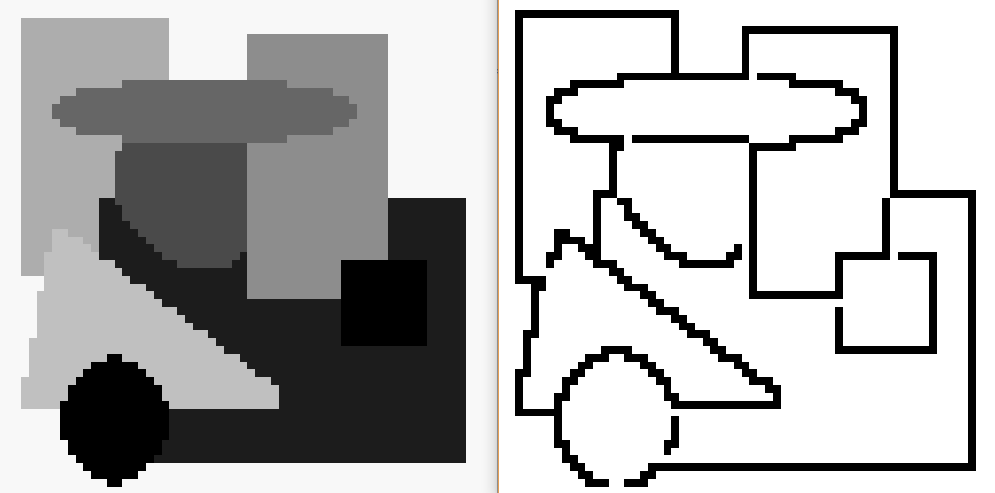
\includegraphics[width=\linewidth]{./Experiments/Template/fig/fig1.png}
\captionof{figure}{This is the Share\LaTeX{} logo}
\end{Figure}


\lipsum[10] 

\begin{Figure}
 \centering
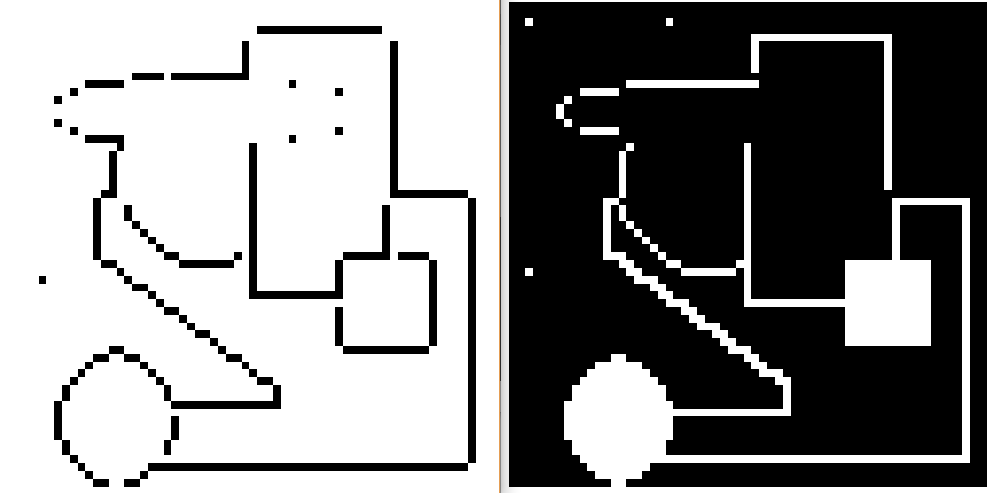
\includegraphics[width=\linewidth]{./Experiments/Template/fig/fig2.png}
\captionof{figure}{This is the Share\LaTeX{} logo}
\end{Figure}

\lipsum[1]

\begin{Figure}
 \centering
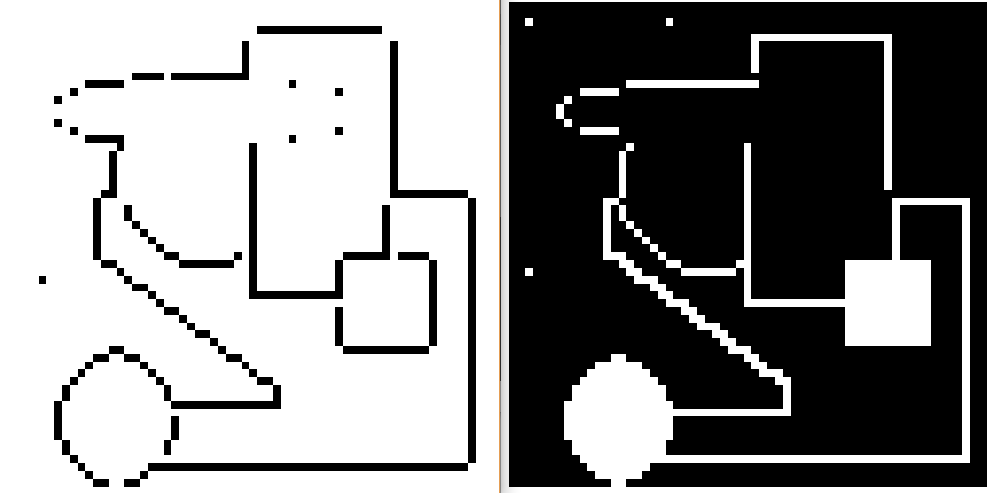
\includegraphics[width=\linewidth]{./Experiments/Template/fig/fig2.png}
\captionof{figure}{This is the Share\LaTeX{} logo}
\end{Figure}

\lipsum[1]
\end{multicols}